\documentclass{article}
\usepackage{amsmath,amsfonts,amsthm,amssymb,amsopn,bm}
\usepackage[margin=.9in]{geometry}
\usepackage{graphicx}
\usepackage{url}
\usepackage[usenames,dvipsnames]{color}
\usepackage{fancyhdr}
\usepackage{multirow}
\usepackage{listings}
\usepackage{hyperref}

\definecolor{keywords}{RGB}{255,0,90}
\definecolor{comments}{RGB}{0,0,113}
\definecolor{red}{RGB}{160,0,0}
\definecolor{green}{RGB}{0,150,0}
 
\lstset{language=Python, 
        basicstyle=\ttfamily\tiny, 
        keywordstyle=\color{keywords},
        commentstyle=\color{comments},
        stringstyle=\color{red},
        showstringspaces=false}

\newcommand{\field}[1]{\mathbb{#1}}
\newcommand{\1}{\mathbf{1}}
\newcommand{\E}{\mathbb{E}} 
\newcommand{\Z}{\mathbb{Z}} 
\renewcommand{\P}{\mathbb{P}}
\newcommand{\R}{\field{R}} % real domain
% \newcommand{\C}{\field{C}} % complex domain
\newcommand{\F}{\field{F}} % functional domain
\newcommand{\T}{^{\textrm T}} % transpose
\def\diag{\text{diag}}

%% operator in linear algebra, functional analysis
\newcommand{\inner}[2]{#1\cdot #2}
\newcommand{\norm}[1]{\left\|#1\right\|}
\newcommand{\twonorm}[1]{\|#1\|_2^2}
% operator in functios, maps such as M: domain1 --> domain 2
\newcommand{\Map}[1]{\mathcal{#1}}
\renewcommand{\theenumi}{\alph{enumi}} 

\newcommand{\Perp}{\perp \! \! \! \perp}

\newcommand\independent{\protect\mathpalette{\protect\independenT}{\perp}}
\def\independenT#1#2{\mathrel{\rlap{$#1#2$}\mkern2mu{#1#2}}}
\newcommand{\vct}[1]{\boldsymbol{#1}} % vector
\newcommand{\mat}[1]{\boldsymbol{#1}} % matrix
\newcommand{\cst}[1]{\mathsf{#1}} % constant
\newcommand{\ProbOpr}[1]{\mathbb{#1}}
\newcommand{\points}[1]{\small\textcolor{magenta}{\emph{[#1 points]}} \normalsize}
\date{{}}

\setlength\parindent{0px}

\begin{document}
\title{Homework \#4}
\author{\normalsize{Winter 2020, STATS 509}\\
\normalsize{Dino Bektesevic}}
\maketitle

\section*{Problem 1}
Suppose that $X$ is a positive random variable so that 
$P(X > 0) = 1$. Prove that for any $t<0$, $M_X(t) = E[e^{tX}] < \infty$.

\emph{Hint: Find a relationship between $e^{tX}$ and $1$, for $t < 0$.
Use the fact that if for all $x$, $g(x) \leq h(x)$ then $\int g(x) dx \leq \int h(x)dx$.}

\begin{align*}
    M_X(t)  &= E[e^{tX}] = \int_{-\infty}^\infty e^{tx} f_X(x) dx \\
    &= \int_0^\infty e^{tx} f_X(x) dx
\end{align*}

For $t<0$:
$$ e^{tx} f_X(x) \leq f_X(x) \forall f_X(x)$$
because $e^{kx}\leq 1 \forall k<0$ so it follows:
\begin{align*}
    \int_0^\infty e^{tx} f_X(x) dx &\leq \int_0^\infty f_X(x) dx \\
     \int_0^\infty e^{tx} f_X(x) dx &\leq P(X>0) \\
      \int_0^\infty e^{tx} f_X(x) dx &\leq 1
\end{align*}




\newpage
\section*{Problem 2.}
Let $X$ be an exponential random variable with parameter $\lambda > 0$.
\begin{enumerate}
    \item Use Chebyshev's inequality to find an upper bound on $Pr(|X- E[X] | \geq k)$

    \begin{align*}
        P(|X-c|) \geq d) &\leq \frac{E[(X-c)^2]}{d^2} \\
        P(|X-\mu|) \geq k) &\leq \frac{E[(X-\mu)^2]}{k^2} \\
        P(|X-\mu|) \geq k) &\leq \frac{V[X]}{k^2} \\
        P(|X-\mu|) \geq k) &\leq \left(\frac{1}{k\lambda}\right)^2
    \end{align*}

    \item Calculate $E[ |X - E[X]|]$ and then use Markov's inequality to find a different upper bound on $Pr(|X- E[X] | \geq k)$.\par
    {\it Hint: first remove the absolute value by splitting the integral into two pieces. Each piece can then be integrated using the Exponential CDF (or just integrating directly) and integration by parts.}
    
    \begin{align*}
        E[|X - E[X]|] &= E[|X - \mu|] = \int_{-\infty}^\infty |x-\mu|f_X(x) dx \\
        &= \int_{0}^\infty |x-\mu|\lambda e^{-\lambda x} dx \\
        &= \int_0^{1/\lambda} \left(\frac{1}{\lambda} - x\right)\lambda e^{-\lambda x} dx 
            + \int_{1/\lambda}^\infty \left(x - \frac{1}{\lambda} \right)\lambda e^{-\lambda x} dx \\
        &= \int_0^{1/\lambda} e^{-\lambda x} dx 
            - \int_0^{1/\lambda} \lambda xe^{-\lambda x} dx
            + \int_{1/\lambda}^\infty \lambda  xe^{-\lambda x} dx 
            - \int_{1/\lambda}^\infty e^{-\lambda x} dx \\
        &= -\frac{e^{-\lambda x}}{\lambda} \bigg|_0^{1/\lambda} 
            + \lambda \frac{\lambda x+1}{\lambda^2}e^{-\lambda x} \bigg|_0^{1/\lambda}
            - \lambda \frac{\lambda x+1}{\lambda^2}e^{-\lambda x} \bigg|_{1/\lambda}^\infty 
            + \frac{e^{-\lambda x}}{\lambda} \bigg|_{1/\lambda}^\infty \\
        &= -\frac{e^{-\lambda x}}{\lambda} \bigg|_0^{1/\lambda} 
            + \lambda \frac{\lambda x+1}{\lambda^2}e^{-\lambda x} \bigg|_0^{1/\lambda}
            - \lambda \left(\frac{\lambda x}{\lambda^2}e^{-\lambda x} + \frac{e^{-\lambda x}}{\lambda^2} \right)\bigg|_{1/\lambda}^\infty 
            + \frac{e^{-\lambda x}}{\lambda} \bigg|_{1/\lambda}^\infty \\
        &= \left(-\frac{1}{e\lambda}+ \frac{1}{\lambda}\right) 
            + \lambda \left(\frac{2}{e\lambda^2} - \frac{1}{\lambda^2} \right) 
            - \lambda \left(0 + 0 - \frac{2}{e\lambda^2} - \frac{1}{\lambda^2}\right) 
            + \left(0 - \frac{1}{e\lambda}\right) \\
        &= -\frac{1}{e\lambda} + \frac{1}{\lambda} 
           + \frac{2}{e\lambda} - \frac{1}{\lambda}  
           + \frac{2}{e\lambda} + \frac{1}{\lambda} 
           - \frac{1}{e\lambda}\\
        &= \frac{2}{e\lambda} + \frac{1}{\lambda} 
    \end{align*}
    Markov's inequality is then:
    $$P(|X-\mu|\geq k) = \frac{1}{2 e \lambda k}$$

    \item[(c)] For which values of $k$ is the bound in (b) lower than that given in (a)?
    
    \begin{align*}
        1 &> \frac{P_b}{P_a}\\
        k &< \frac{2e}{\lambda} \approx \frac{5.44}{\lambda}
    \end{align*}
\end{enumerate}



\newpage
\section*{Problem 3} 
If the joint probability density of the two random variables $X$ and $Y$ is given by:
$$ f_{XY}(x,y) =\left\{
    \begin{array}{ll}
        2 & \hbox{for } 0 < x < y <1 \\
        0 & \hbox{otherwise.}
    \end{array}
\right.$$

\begin{enumerate}
    \item Find $P(Y<0.5)$. {\it Hint: Draw a graph.}  

    \begin{align*}
        P(Y<0.5) &= \int_0^{0.5} \int_0^y f(x,y)dxdy \\
        &= \int_0^{0.5} \int_0^y 2 dxdy = 2 \frac{y^2}{2}\bigg |_0^{0.5} \\
        &= \frac{1}{4}
    \end{align*}


    \item Find $P(X<0.5)$. 
    
    \begin{align*}
        P(X<0.5) &= \int_0^{0.5}\int_x^1 f(x,y)dydx \\
        &= \int_0^1 (2-2x) dx = 2x|_0^{0.5} -  2\frac{x^2}{2}\bigg |_0^{0.5} \\
        &= 1 - \frac{1}{4} = \frac{3}{4}
    \end{align*}
    
    
    \item Find $P(X+Y < 1)$ 
    
    \begin{align*}
        P(X+Y<1) &= \int_0^{0.5}\int_x^{1-x} f(x,y)dydx \\
        &= 2\int_0^{0.5} (1-2x) dx = 2\left(x|_0^{0.5} -  2\frac{x^2}{2}\bigg |_0^{0.5}\right) \\
        &= 2\frac{1}{4} = \frac{1}{2}
    \end{align*}
        
    
    \item Find the joint CDF $F(x,y)$. {\it (You will need to consider several cases.)}  
    $$F(x,y) = \begin{cases} 
	        0   &\mbox{if } x < 0 \mbox{ or } y<0   \\
	        0   &\mbox{if } y > 1 \mbox{ or } x > y \\
            2xy &\mbox{if } y < 1 \mbox{ and } x<y
        \end{cases}  
    $$
\end{enumerate}




\newpage
\section*{Problem 4} 
Suppose that $X$ and $Y$ are continuous random variables with the following joint cdf:

\begin{equation}\label{eq:one}
F_{XY}(x,y) = \widetilde{F}(x)\widetilde{F}(y)
\end{equation}

where $\widetilde{F}(\cdot)$ is a (univariate) cdf. 

{{(Aside)} \it It follows from {\rm (\ref{eq:one})} that $X$ and $Y$ are independent random variables with the same
marginal distribution.} 

\begin{itemize}
    \item[(a)] For a fixed value $t$, express $P(X \leq t, Y \leq t)$ in terms of $\widetilde{F}(\cdot)$.\par
    {\it Hint: Recall the definition of  a joint cdf $F_{XY}(x,y)$.}
    
    By definition $F(x,y)= P(X\leq x, Y\leq y)$ so it follows that:
    $$P(X \leq t, y\leq t) = F_{XY}(t,t) = \Tilde{F}(t)\Tilde{F}(t) = \Tilde{F}^2(t)$$
    
    \item[(b)] Let $T= \max (X,Y)$. Using your answer to (a) find the cdf $F_T(t)$ and the pdf $f_T(t)$ for $T$:\par
    {\it Hint: If $X\leq t$ {\bf and} $Y\leq t$, what can one say about $\max(X,Y)$}?
    
    For $T\leq t$ to hold both $X\leq t$ and $Y\leq t$ have to be satisfied. This is by definition the case for a CDF, so then the joint CDF is just
    
    $$ F_T(t) = \Tilde{F}^2(t)$$
    
    By definition the PDF:
    
    \begin{align*}
        f_T(t) = \frac{\partial}{\partial t} F_T(t) &=  \frac{\partial}{\partial t} \Tilde{F}^2(t) \\
        &= 2\Tilde{F}(t)\Tilde{f(t)}
    \end{align*}

\end{itemize}




\newpage
\section*{Problem 5}  If the joint CDF for two random variables, $X$ and $Y$, is  
given by:
$$
F_{XY}(x,y) = \begin{cases}
    (1-e^{-x^2})(1-e^{-y^2}) & \hbox{for } x>0, y>0\\[4pt]
    0 & \hbox{otherwise}
    \end{cases}
$$
Find the joint pdf $f_{XY}(x,y)$.

\begin{align*}
    \frac{\partial^2}{\partial x \partial y} F(x,y) &=  \frac{\partial^2}{\partial x \partial y} (1-e^{-x^2})(1-e^{-x^2}) \\
    &= \frac{\partial}{\partial x} \left[ (1-e^{-x^2}) 2ye^{-y^2} \right] \\
    &=  2xe^{-x^2} 2ye^{-y^2} \\
    &= 4 xy e^{-(x^2+y^2)}
\end{align*}



\newpage
\section*{Problem 6}  Let $X$ and $Y$ have the joint density function (here $k>0$ is an unknown constant):
$$ f_{XY}(x,y) = \begin{cases}
    k(x-y), & 0\leq y\leq x \leq 1;\\[4pt]
    0 & \hbox{otherwise,}
\end{cases}$$

\begin{enumerate}
    \item Sketch the support of the joint density. You will need to use this in answering the next three question parts.
    
    \begin{center}
    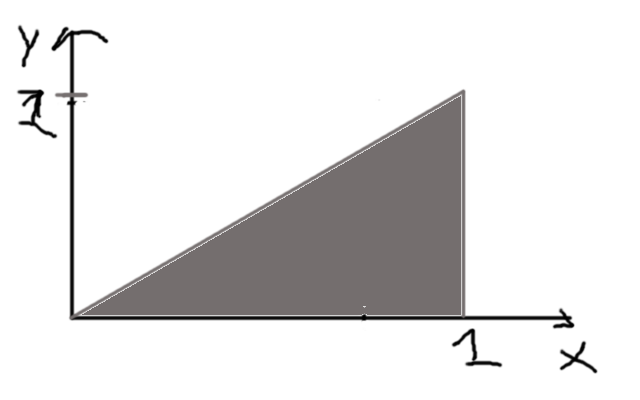
\includegraphics[width=200px]{STATS509/HW4/HW4Figures/picasso4.png}
    \end{center}

    \item Find the constant of proportionality $k$.
    
    \begin{align*}
    1 &= \int_0^1\int_0^x k(x-y)dydx\\
      &= k \int_0^1 \left[xy - \frac{y^2}{2}\right]\bigg |_0^x dx \\
      &= k \int_0^1 \left[x^2 - \frac{x^2}{2}\right] dx \\
      &= k \left[ \frac{x^3}{3} - \frac{1}{2}\frac{x^3}{3} \right] \bigg |_0^1 \\
      &= k \left( \frac{1}{3} - \frac{1}{6}\right) = \frac{k}{6}\\
    k &= 6
    \end{align*}

    \item Find the marginal densities $f_X(x)$ and $f_Y(y)$.
    
    \begin{align*}
    f_X(x) &= \int_0^1 6(x-y) dy \\
    &= \left[6xy - 3y^2\right]\bigg|_0^1 \\
    &= 6x-3
    \end{align*}
    
    \begin{align*}
    f_Y(y) &= \int_0^1 6(x-y) dx \\
    &= \left[3x^2 - 6yx\right]\bigg|_0^1 \\
    &= 3 - 6y
    \end{align*}

    \newpage
    \item Find the conditional densities of $f_{Y|X}(y\mid x)$ and $f_{X|Y}(x\mid y)$.\par
    Remember to carefully state for which values of the conditioning variable these are defined.
    
    By definition : $f_{Y\mid X}(y \mid x) = \frac{f_{X, Y}(x, y)}{f_X(x)}$. So on $0\leq x \leq 1$ we have:
    $$ f_{Y\mid X}(y \mid x) = \frac{6(x-y)}{6x-3} = \frac{2(x-y)}{2x-1} $$
    and on $0\leq y\leq 1 $ we have:
    $$ f_{X\mid Y}(x \mid y) = \frac{6(x-y)}{3-6y} = \frac{2(x-y)}{1-3y} $$
   
\end{enumerate}



\newpage
\section*{Problem 7} 
If the joint probability density of the two random variables $X$ and $Y$ is given by:
$$ f_{XY}(x,y) = \begin{cases}
    4xy & \hbox{for } 0 < y<1,\; 0<x <1,\\
    0 & \hbox{otherwise.}
    \end{cases}$$
Let $D=(X-Y)$ and $S=(X+Y)$.  

\begin{enumerate}
    \item Solve for $X$  and $Y$ in terms of $D$ and $S$.

    \begin{align*}
        D + S &= X - Y + X + Y \\
        D + S &= 2X \\
        X &= \frac{D + S}{2}
    \end{align*}

    \begin{align*} 
        y = S - \frac{D + S}{2} \\
        y = \frac{S - D}{2}
    \end{align*}

    \item Find the support of $f_{DS}(d,s)$ and draw a sketch.
    
    \begin{center}
    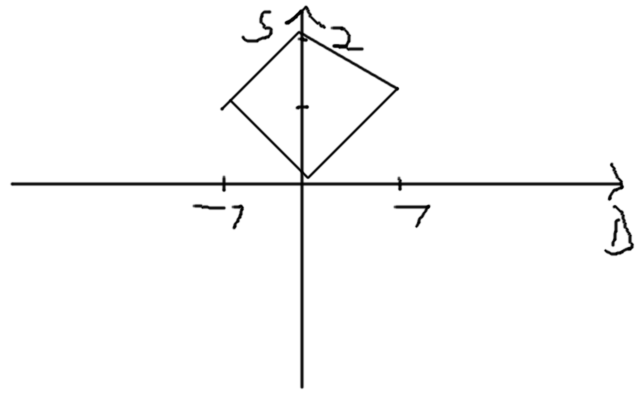
\includegraphics[width=200px]{STATS509/HW4/HW4Figures/picasso4aa.png}
    \end{center}
    
    The boundary lines are given by the following equations, left to right in a clockwise direction:
    \begin{align*}
        s &= -d \\
        s &= d+2 \\
        s &= -d+2 \\
        s &= d
    \end{align*}
    where we notice that boundaries are symmetrical around $s=0$. 
    
    \newpage
    \item Find the joint pdf $f_{DS}(d,s)$.
    
    By definition:
    $$f_{DV}(d,v) = f_{XY}(g_1(x,y), g_2(x,y)) |J|$$
    where $g_1(x,y)=0.5(D+S)$, $g_2(x,y)=0.5(S-D)$ and:
    
    \begin{align*}
    J &= \begin{vmatrix}
        \frac{\partial x}{\partial d} & \frac{\partial y}{\partial d} \\ 
        \frac{\partial x}{\partial v} & \frac{\partial y}{\partial v}
        \end{vmatrix} 
     = \begin{vmatrix}
        \frac{1}{2} & -\frac{1}{2} \\ 
        \frac{1}{2} & \frac{1}{2}
        \end{vmatrix} \\
    &= \frac{1}{4} + \frac{1}{4} \\
    &= - \frac{1}{2}
    \end{align*}
    
    So putting it all back into the definition:
    
    \begin{align*}
     f_{DS}(u,v) &= f_{XY}\left(\frac{D + S}{2}, \frac{S - D}{2}\right) \bigg|\frac{1}{2}\bigg| \\
     &= \frac{1}{2} f_{XY}\left(\frac{D + S}{2}, \frac{S - D}{2}\right) \\
     &= \begin{cases}
        \frac{1}{2} 4\frac{s+d}{2}\frac{s-d}{2} = s^2-d^2 & \hbox{ when inside the diamond } \\ 
        0 & \hbox{otherwise.}
        \end{cases}
    \end{align*}

    \newpage
    \item Find the marginal densities $f_D(d)$ and $f_S(s)$.
    
    \begin{align*}
    f_{D}(d) &= \int_{-\infty}^\infty s^2 - d^2 ds \\
    &= \begin{cases}
       \int_{-d}^{d+2} s^2 - d^2 ds &\hbox{ for } -1 < d < 0, \\
       \int_{d}^{2-d} s^2 - d^2 ds  &\hbox{ for } 0\leq d < 1 \\
       0 &\hbox{otherwise.}
       \end{cases}
    \end{align*}
    
    Let's split the integrals out for simplicity:

    \begin{align*}
        \int_{-d}^{d+2} s^2 - d^2 ds &=  \int_{-d}^{d+2} s^2 ds -  d^2\int_{-d}^{d+2} ds \\
        &= \frac{s^3}{3}\bigg |_{-d}^{d+2} - d^2 s|_{-d}^{d+2} \\
        &= \frac{(d+2)^3}{3} - \frac{-d^3}{3} - d^2(2d+2) \\
        &= \frac{(d+2)^3}{3} - \frac{5}{3} d^3 - 2d^2
    \end{align*}
    
    and
    
    \begin{align*}
        \int_{d}^{2-d} s^2 - d^2 ds &=  \int_{d}^{2-d} s^2 ds -  d^2\int_{d}^{2-d} ds \\
        &= \frac{s^3}{3}\bigg |_{d}^{2-d} - d^2 s|_{d}^{2-d} \\
        &= \frac{(2-d)^3}{3} - \frac{d^3}{3} - d^2(2-2d) \\
        &= \frac{(d+2)^3}{3} - \frac{7}{3} d^3 - 2d^2 
    \end{align*}
    
    So in the end:
    
    \begin{align*}
    f_{D}(d) &= \int_{-\infty}^\infty s^2 - d^2 ds \\
    &= \begin{cases}
       \frac{(d+2)^3}{3} - \frac{5}{3} d^3 - 2d^2 &\hbox{ for } -1 < d < 0, \\
       \frac{(d+2)^3}{3} - \frac{7}{3} d^3 - 2d^2   &\hbox{ for } 0\leq d < 1 \\
       0 &\hbox{otherwise.}
       \end{cases}
    \end{align*}
    
    \newpage
    We repeat the same for $f_{S}(s)$ and get something like:
    
    \begin{align*}
    f_{S}(s) &= \int_{-\infty}^\infty s^2 - d^2 dd \\
    &= \begin{cases}
       \int_{s-2}^{2-s} s^2 - d^2 dd &\hbox{ for } 1 < s < 2, \\
       \int_{-s}^{s} s^2 - d^2 dd  &\hbox{ for } 0 < s\leq 1 \\
       0 &\hbox{otherwise.}
       \end{cases} \\
    &= \begin{cases}
       4s^2 - 2s^3 - \frac{2}{3}(2-s)^3 &\hbox{ for }  1 < s < 2, \\
       \frac{4}{3}s^3  &\hbox{ for } 0 < s\leq 1 \\
       0 &\hbox{otherwise.}
       \end{cases} \\
    \end{align*}
    
    
    \item Find the conditional densities of $f_{D|S}(d\mid s)$ and $f_{S|D}(s\mid d)$.\par
    Remember to carefully state for which values of the conditioning variable these are defined.
    
    We follow the definition: 
    
    $$f_{Y\mid X}(y \mid x) = \frac{f_{X, Y}(x, y)}{f_X(x)}$$
    
    Note that life is worth living so we leave writing out the expressions explicitly to the reader.
    
    
\end{enumerate}



\newpage
\section*{Problem 8} The random variables $(X,Y)$ have the following joint pdf:
$$f_{XY}(x,y) = \begin{cases}
    2y & \hbox{for } 0 < x < 1 \hbox{ and } 0 < y <1,\\ 
    0 & \hbox{otherwise.}
    \end{cases}
$$
Consider the transformation: $U = XY$ and $ V=X$.

\begin{enumerate}
    \item Draw the support of the joint density $f_{XY}(x,y)$ for $(X,Y)$.
    
    \begin{center}
    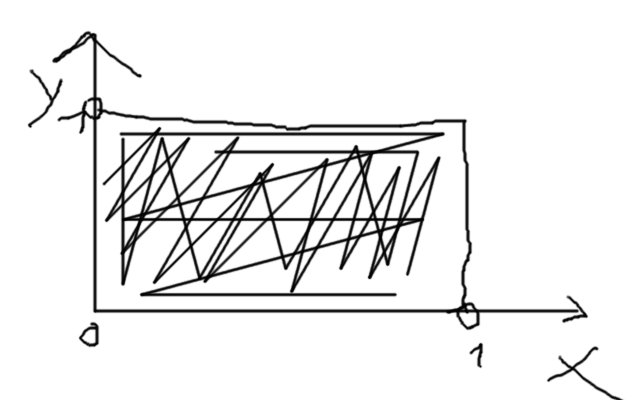
\includegraphics[width=200px]{STATS509/HW4/HW4Figures/picasso4a.png}
     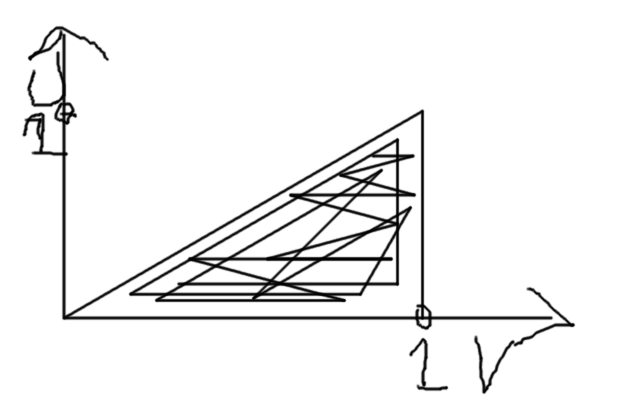
\includegraphics[width=200px]{STATS509/HW4/HW4Figures/picasso4b.png}
    \end{center}

    \item Solve for $X$ and $Y$ in terms of $U$ and $V$.

    $$V=X \rightarrow X=V$$
    $$U=XY \rightarrow Y=\frac{U}{V}$$    
    
    \item Carefully find the support for the joint density for $(U,V)$. Then find the joint density $f_{UV}(u,v)$, remember to include the support.
    
    By definition:
    $$f_{UV}(u,v) = f_{XY}(g_1(x,y), g_2(x,y)) |J|$$
    where $g_1(x,y)=v$, $g_2(x,y)=u/v$ and:
    
    \begin{align*}
    J &= \begin{vmatrix}
        \frac{\partial x}{\partial u} & \frac{\partial y}{\partial u} \\ 
        \frac{\partial x}{\partial v} & \frac{\partial y}{\partial v}
        \end{vmatrix} 
     = \begin{vmatrix}
        0 & \frac{1}{v} \\ 
        1 & -\frac{u}{v^2}
        \end{vmatrix} \\
    &= 0\cdot -\frac{u}{v^2} - \frac{1}{v}\cdot 1 \\
    &= - \frac{1}{v}
    \end{align*}
    
    So putting it all back into the definition:
    
    \begin{align*}
     f_{UV}(u,v) &= f_{XY}\left(v, \frac{u}{v}\right) \bigg|- \frac{1}{v}\bigg| \\
     &= \frac{1}{v} f_{XY}\left(v, \frac{u}{v}\right) \\
     &= \begin{cases}
        \frac{1}{v} 2\frac{u}{v} = 2\frac{u}{v^2} & \hbox{for } 0 < u < v < 1\\ 
        0 & \hbox{otherwise.}
        \end{cases}
    \end{align*}
    
    \item Find the marginal densities $f_U(u)$ for $U$ and  $f_V(v)$ for $V$.
    
    \begin{align*}
    f_{U}(u) &= \int_u^1 \frac{2u}{v^2} dv \\
    &= 2u \left(-\frac{1}{v}\bigg|_u^1\right) \\
    &= 2u(\frac{1}{u} - 1) = 2 - 2u \\
    &= 2(1-u)
    \end{align*}
     
    \begin{align*}
    f_{V}(v) &= \int_0^v \frac{2u}{v^2} du \\
    &= \frac{2}{v^2} \frac{u^2}{2}\bigg|_0^v \\
    &= \frac{2}{v^2} \frac{v^2}{2} = 1
    \end{align*}
     
\end{enumerate}


\end{document}
